\documentclass{llncs}

\usepackage{forest}
\usepackage[utf8]{inputenc}
\usepackage{listings}
\usepackage{hyperref}

\graphicspath{{./img_t2/}}


\definecolor{folderbg}{RGB}{124,166,198}
\definecolor{folderborder}{RGB}{110,144,169}
\def\Size{4pt}
\tikzset{
      folder/.pic={
        \filldraw[draw=folderborder,top color=folderbg!50,bottom color=folderbg]
          (-1.05*\Size,0.2\Size+5pt) rectangle ++(.75*\Size,-0.2\Size-5pt);  
        \filldraw[draw=folderborder,top color=folderbg!50,bottom color=folderbg]
          (-1.15*\Size,-\Size) rectangle (1.15*\Size,\Size);
      }
    }





\begin{document}

\title{Relatório do Trabalho 2}
\author{Gustavo Henrique Fernandes Carvalho - 14/0021671}
\institute{Fundamentos Computacionais de Robótica - 2017/2 - Universidade de Brasília}
\maketitle


O video da simulação está em \url{https://youtu.be/T5etANWVPl0}


\section{Informações do pacote}
\subsection{Dependências}
Para executar a simulação do trabalho 2 não é necessário nenhuma dependência além das dependências originais do pacote fcr2017, definidas no arquivo \textit{package.xml}.


\subsection{Rodando a simulação}
Para rodar a simulação é necessário apenas executar o seguinte comando no terminal:
\begin{lstlisting}[language=bash]
	$ roslaunch fcr2017 trabalho2.launch
\end{lstlisting}
O arquivo \textit{trabalho2.launch} já inicia todos os nós necessários para a simulação, inclusive o nó de controle do trabalho 2.

A simulação é dividida em 3 etapas, na primeira etapa o Pioneer se move para uma posição inicial no mapa topológico definida pelo usuário, na segunda etapa o Pioneer percorre todo o mapa topológico preenchendo a grade de ocupação de cada região do mapa, e na última etapa o Pioneer vai para a posição final também  definida pelo usuário, as interfaces de entrada e saída da simulação são explicadas com mais detalhes nas seções \ref{sec:entrada} e \ref{sec:saida}.


\subsection{Arquivos}
A Figura \ref{file_tree} mostra os novos arquivos do pacote fcr2017 utilizados para a realização do trabalho 2, os arquivos originais do pacote não são mostrados.

\pagebreak
\begin{figure}[h!]
\begin{forest}
      for tree={
        font=\ttfamily,
        grow'=0,
        child anchor=west,
        parent anchor=south,
        anchor=west,
        calign=first,
        inner xsep=7pt,
        edge path={
          \noexpand\path [draw, \forestoption{edge}]
          (!u.south west) +(7.5pt,0) |- (.child anchor) pic {folder} \forestoption{edge label};
        },
        % style for your file node 
        file/.style={edge path={\noexpand\path [draw, \forestoption{edge}]
          (!u.south west) +(7.5pt,0) |- (.child anchor) \forestoption{edge label};},
          inner xsep=2pt,font=\scriptsize\ttfamily
                     },
        before typesetting nodes={
          if n=1
            {insert before={[,phantom]}}
            {}
        },
        fit=band,
        before computing xy={l=15pt},
      }  
	[fcr2017
		[launch
			[trabalho2.launch - Utilizado para iniciar a simulação, file]
			[trabalho2.rviz - Configuração do RViz, file]
			[..., file]
		]
		[map\_output - Diretório onde as imagens das grades de ocupação são salvas.
		]
		[src
			[140021671\_Trabalho2.cpp - Código fonte do trabalho 2, file]
			[common\_lib - Biblioteca implementada para facilitar o reuso e modificação do código
				[common.cpp - Implementação de funções gerais, file]
				[common.h - Definição de funções e estruturas gerais, file]
				[graph.cpp - Implementação das funções para manipulação de grafo, file]
				[graph.h - Definição das funções e estruturas para manipulação de grafo, file]
				[grid\_map.cpp - Implementação das funções que fazem a grade de ocupação, file]
				[grid\_map.h - Definição das funções e estruturas que fazem a grade de ocupação, file]
				[laser\_sensor.cpp - Implementação das funções que manipulam os dados do sensor laser, file]
				[laser\_sensor.h - Definição das funções e estruturas que manipulam os dados do sensor laser, file]
				[motion\_controller.cpp - Implementação das funções de controle de movimento, file]
				[motion\_controller.h - Definição das funções e estruturas de controle de movimento, file]
				[odometer.cpp - Implementação das funções manipulam os dados do odômetro, file]
				[odometer.h - Definição das funções e estruturas manipulam os dados do odômetro, file]
			]
		]
		[CIC\_graph.txt - Definição do mapa topológico do primeiro andar do prédio CIC/EST, file]
		[README.txt - Mais informações sobre o pacote, file]
		[..., file]
	]
\end{forest}
\caption{Estrutura dos arquivos.}
\label{file_tree}
\end{figure}


\section{Entrada de dados} \label{sec:entrada}
Toda a entrada de dados pelo usuário é feita pelo terminal, a simulação requer apenas dois dados de entrada do usuário, o nó inicial e o final, utilizados na primeira e última etapa da simulação respectivamente.

A entrada desses dois nós é feita de maneira semelhante, uma mensagem indicando que o programa está esperando o usuário digitar um nó é mostrada no terminal e a mensagem continua aparecendo até o usuário digitar um nó válido do mapa topológico como mostrado nas Figuras \ref{fig:inicial} e \ref{fig:final}.

\begin{figure}[h]
	\centering
	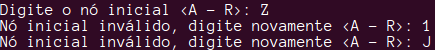
\includegraphics[scale=0.75]{no_inicial}
	\caption{Entrada do nó inicial}
	\label{fig:inicial}
\end{figure}
\begin{figure}[h]
	\centering
	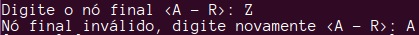
\includegraphics[scale=0.75]{no_final}
	\caption{Entrada do nó final}
	\label{fig:final}
\end{figure}


\section{Saída de dados} \label{sec:saida}
As informações da simulação são apresentadas por 4 interfaces diferentes, descritas individualmente a seguir.

\subsection{Gazebo}
O Gazebo mostra o estado da simulação graficamente e em tempo real da simulação.

\subsection{RViz}
O RViz mostra a leitura dos sensores do Pioneer e a grade de ocupação, ambos atualizados em tempo real, como mostra a Figura \ref{fig:rviz}.

\begin{figure}
	\centerline{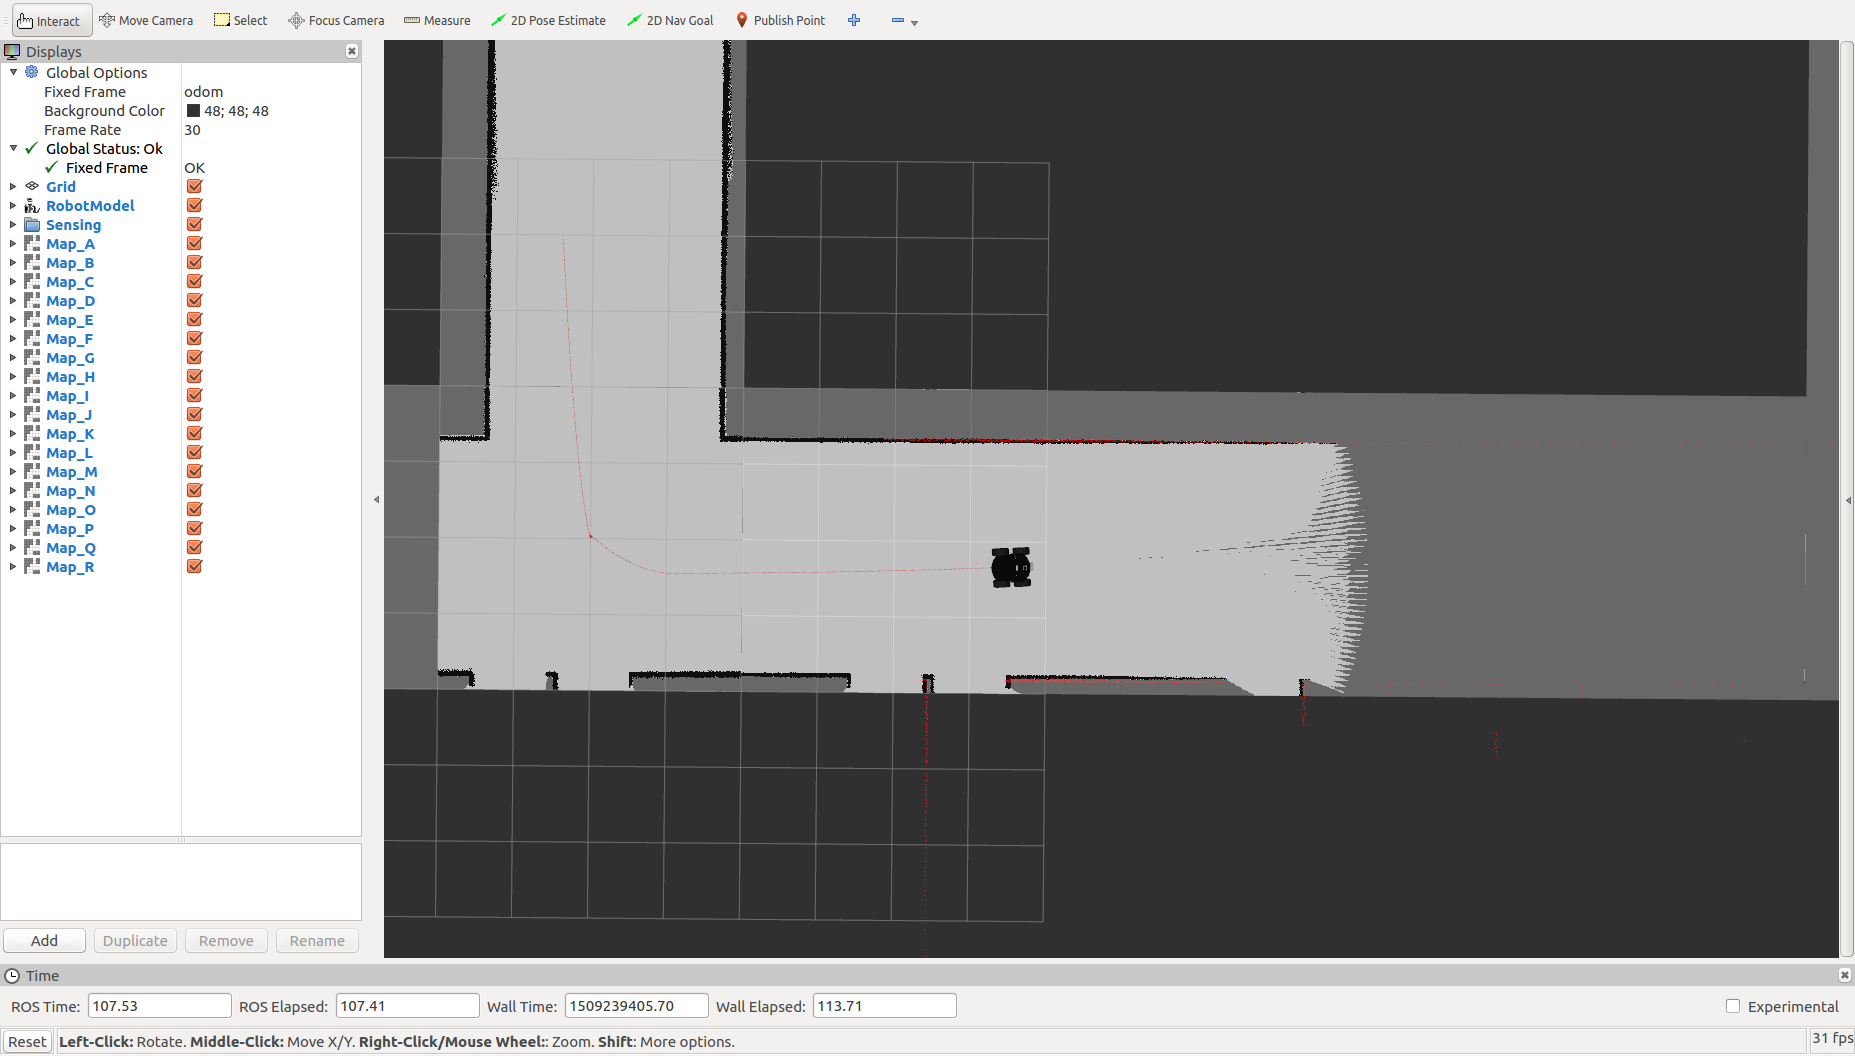
\includegraphics[scale=0.27]{rviz}}
	\caption{Simulação no RViz}
	\label{fig:rviz}
\end{figure}


\subsection{Terminal}
Informações sobre o que o Pioneer está fazendo são atualizados constantemente no terminal informando a localização, para onde ele está indo e qual etapa da simulação ele está, a figura \ref{fig:terminal} mostra um exemplo dessas mensagens.

\begin{figure}
	\centerline{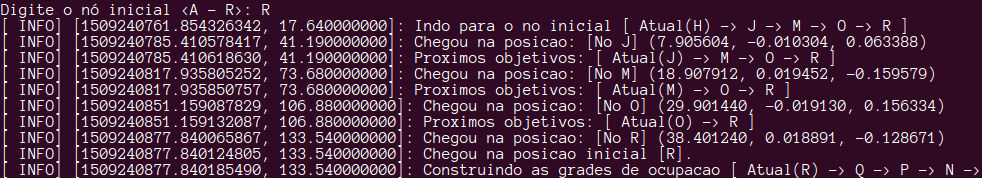
\includegraphics[scale=0.5]{terminal}}
	\caption{Mensagens de atualização pelo terminal}
	\label{fig:terminal}
\end{figure}


\pagebreak
\subsection{Arquivos das grades de ocupação}
Quando as grades de ocupação de todas as regiões do mapa topológico estão completas, elas são salvas como imagens na pasta \textit{map\_output/}. As imagens correspondente a cada um dos nós do grafo são mostrados nas Figuras \ref{fig:grade_no_A} a \ref{fig:grade_no_R}.

\begin{figure}
	\centering
	\fbox{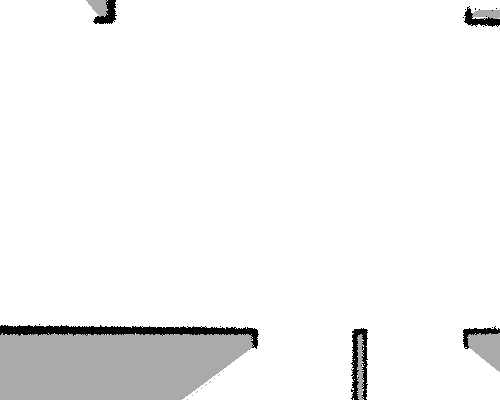
\includegraphics[scale=0.25]{cic_node_A}}
	\caption{Grade de ocupação do nó A}
	\label{fig:grade_no_A}
\end{figure}
\begin{figure}
	\centering
	\fbox{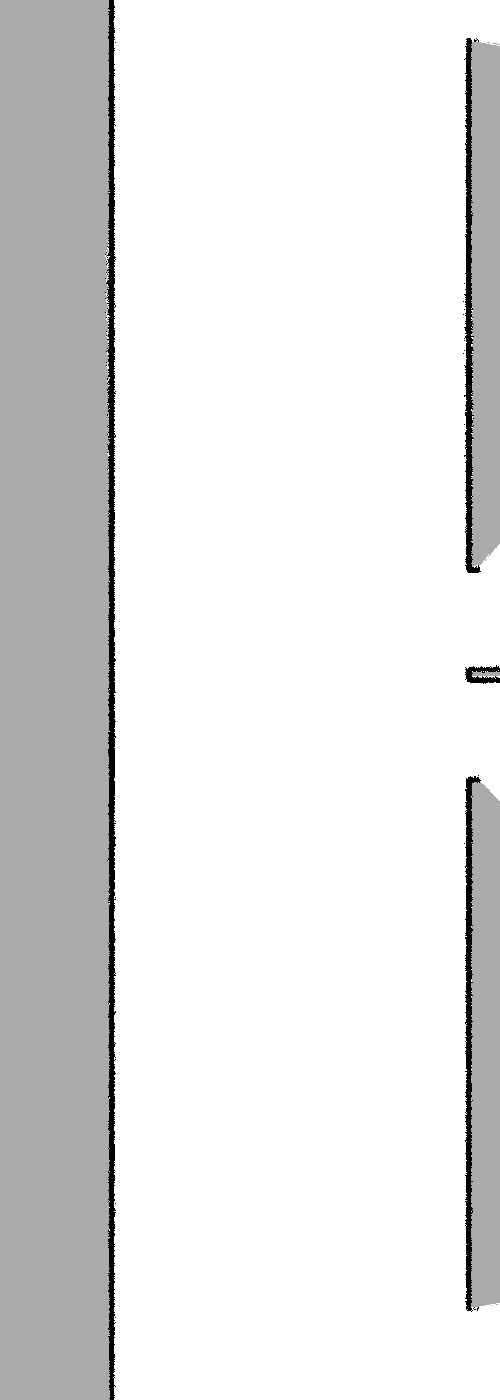
\includegraphics[angle=90,scale=0.25]{cic_node_B}}
	\caption{Grade de ocupação do nó B}
	\label{fig:grade_no_B}
\end{figure}
\begin{figure}
	\centering
	\fbox{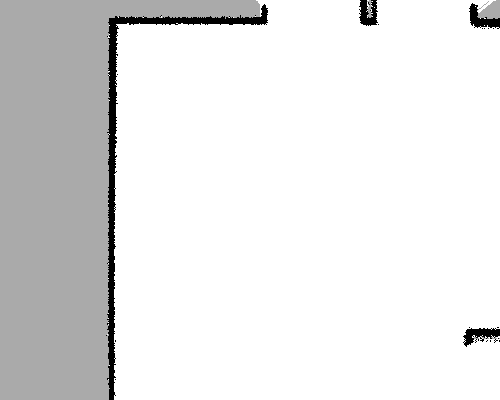
\includegraphics[scale=0.25]{cic_node_C}}
	\caption{Grade de ocupação do nó C}
	\label{fig:grade_no_C}
\end{figure}
\begin{figure}
	\centering
	\fbox{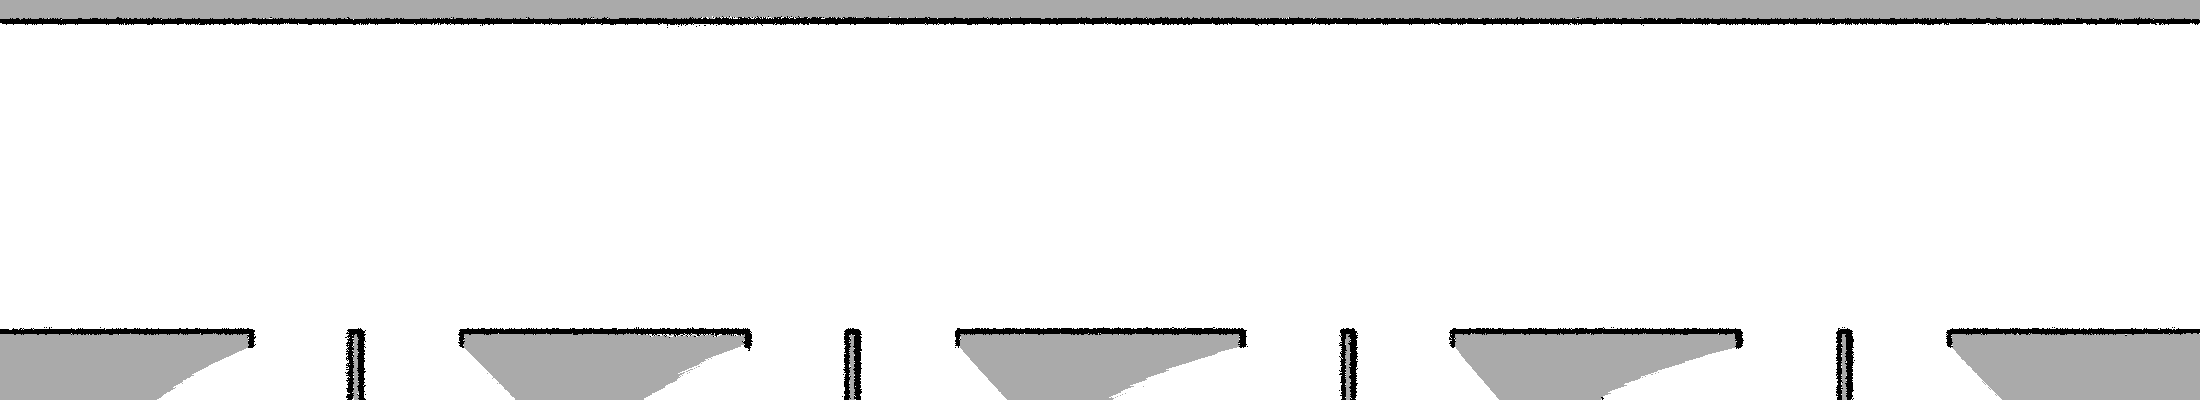
\includegraphics[scale=0.2]{cic_node_D}}
	\caption{Grade de ocupação do nó D}
	\label{fig:grade_no_D}
\end{figure}
\begin{figure}
	\centering
	\fbox{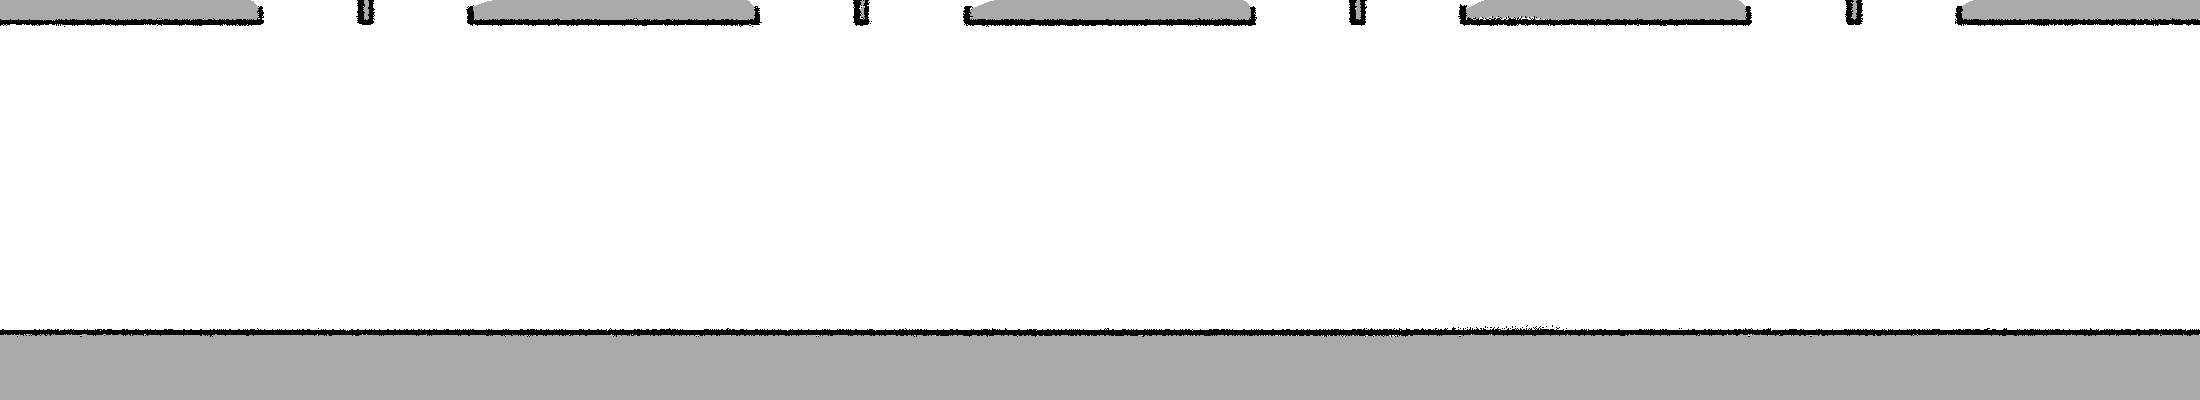
\includegraphics[scale=0.2]{cic_node_E}}
	\caption{Grade de ocupação do nó E}
	\label{fig:grade_no_E}
\end{figure}
\begin{figure}
	\centering
	\fbox{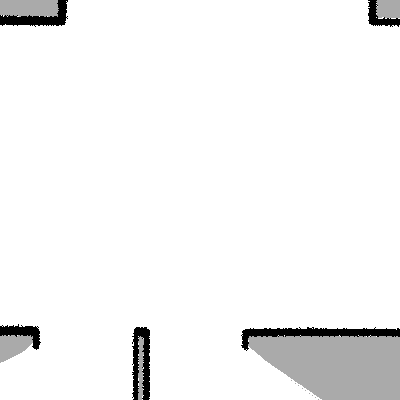
\includegraphics[scale=0.25]{cic_node_F}}
	\caption{Grade de ocupação do nó F}
	\label{fig:grade_no_F}
\end{figure}
\begin{figure}
	\centering
	\fbox{
\includegraphics[angle=90,scale=0.25]{cic_node_G}}
	\caption{Grade de ocupação do nó G}
	\label{fig:grade_no_G}
\end{figure}
\begin{figure}
	\centering
	\fbox{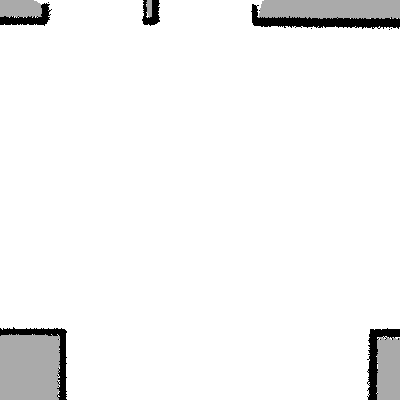
\includegraphics[scale=0.25]{cic_node_H}}
	\caption{Grade de ocupação do nó H}
	\label{fig:grade_no_H}
\end{figure}
\begin{figure}
	\centering
	\fbox{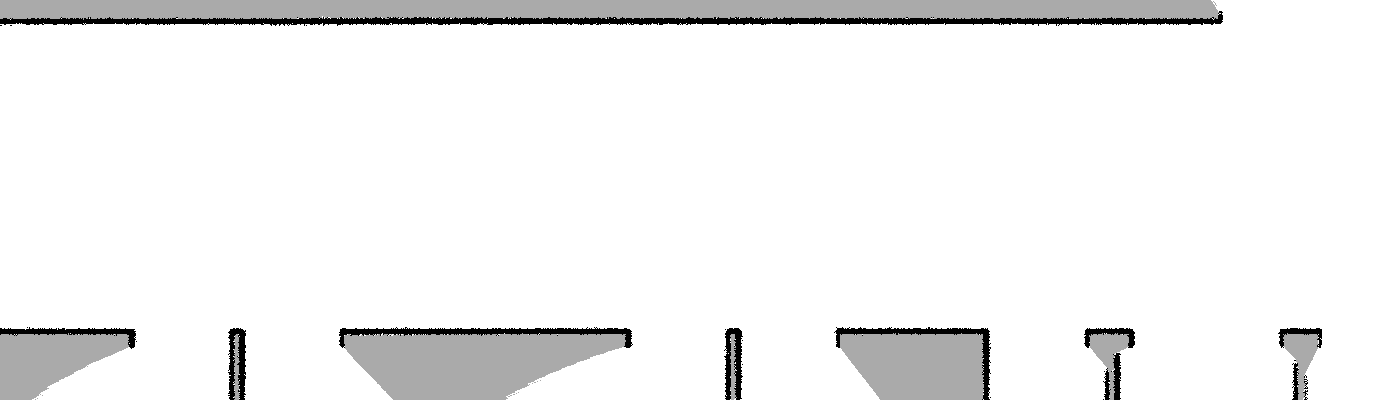
\includegraphics[scale=0.25]{cic_node_I}}
	\caption{Grade de ocupação do nó I}
	\label{fig:grade_no_I}
\end{figure}
\begin{figure}
	\centering
	\fbox{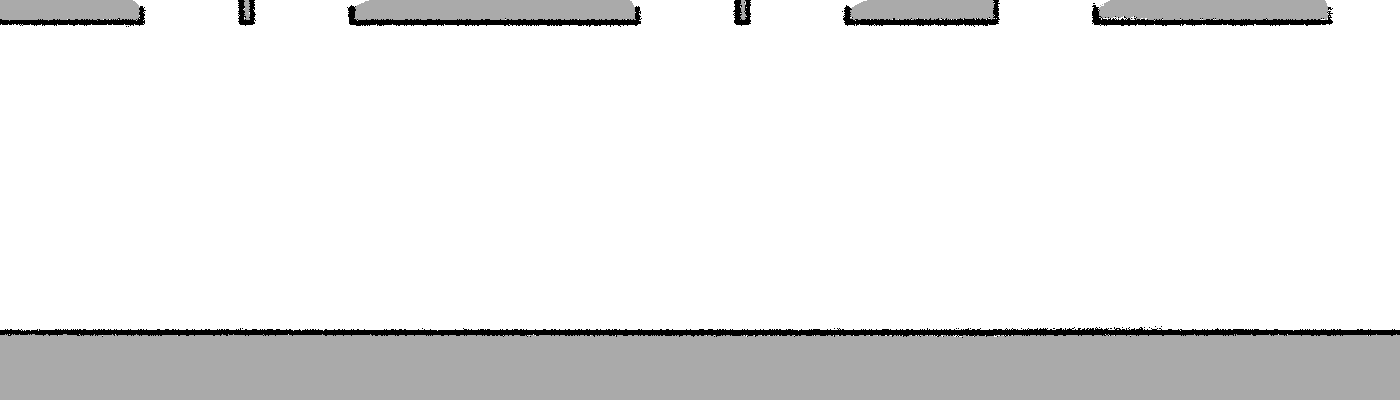
\includegraphics[scale=0.25]{cic_node_J}}
	\caption{Grade de ocupação do nó J}
	\label{fig:grade_no_J}
\end{figure}
\begin{figure}
	\centering
	\fbox{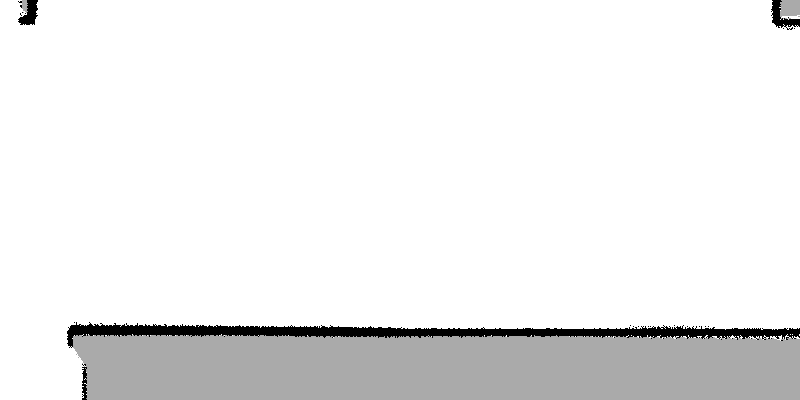
\includegraphics[scale=0.25]{cic_node_K}}
	\caption{Grade de ocupação do nó K}
	\label{fig:grade_no_K}
\end{figure}
\begin{figure}
	\centering
	\fbox{
\includegraphics[angle=90,scale=0.25]{cic_node_L}}
	\caption{Grade de ocupação do nó L}
	\label{fig:grade_no_L}
\end{figure}
\begin{figure}
	\centering
	\fbox{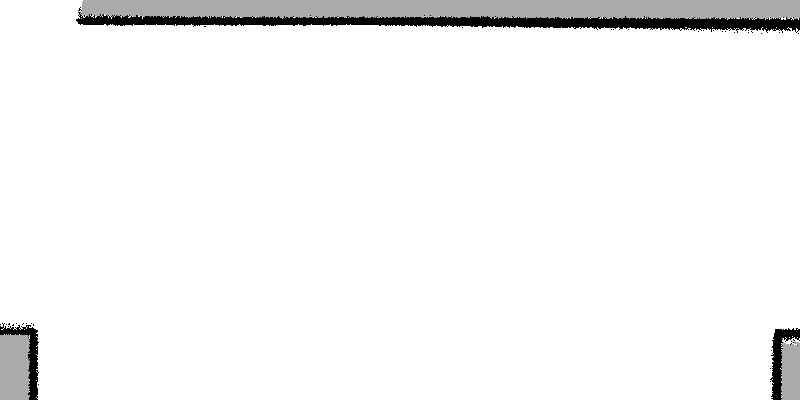
\includegraphics[scale=0.25]{cic_node_M}}
	\caption{Grade de ocupação do nó M}
	\label{fig:grade_no_M}
\end{figure}
\begin{figure}
	\centering
	\fbox{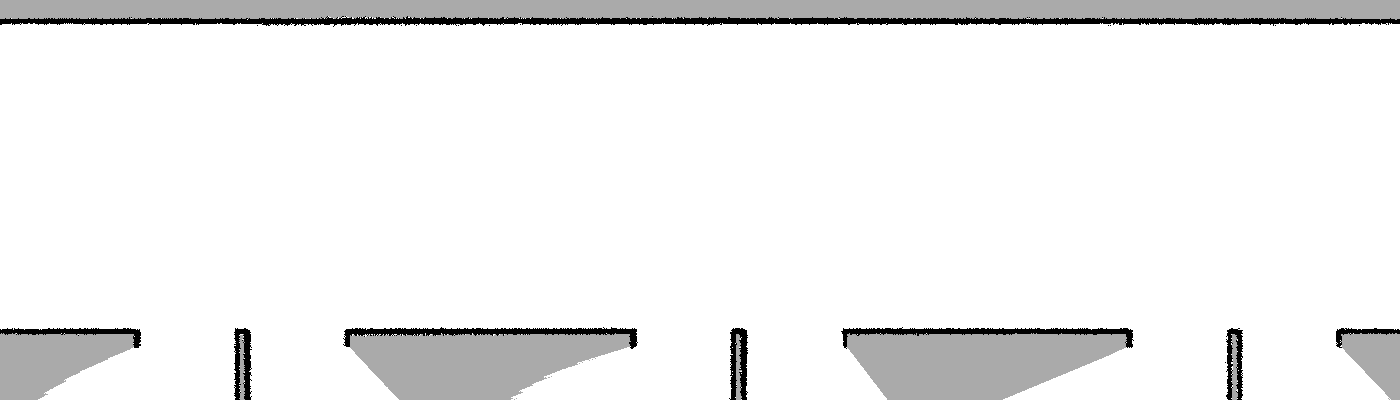
\includegraphics[scale=0.25]{cic_node_N}}
	\caption{Grade de ocupação do nó N}
	\label{fig:grade_no_N}
\end{figure}
\begin{figure}
	\centering
	\fbox{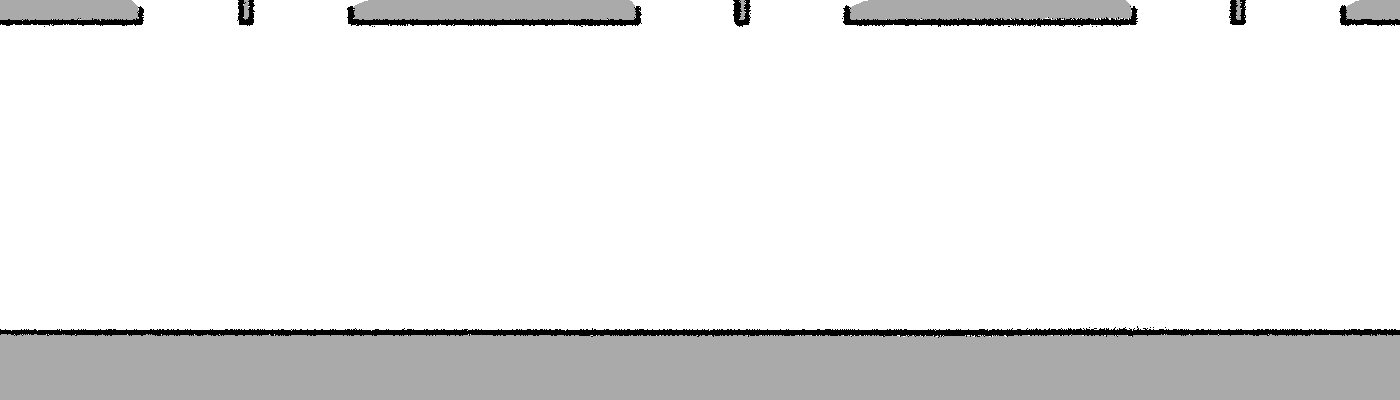
\includegraphics[scale=0.25]{cic_node_O}}
	\caption{Grade de ocupação do nó O}
	\label{fig:grade_no_O}
\end{figure}
\begin{figure}
	\centering
	\fbox{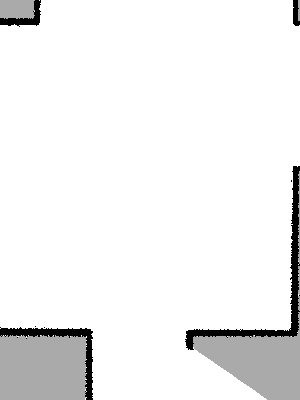
\includegraphics[scale=0.25]{cic_node_P}}
	\caption{Grade de ocupação do nó P}
	\label{fig:grade_no_P}
\end{figure}
\begin{figure}
	\centering
	\fbox{
\includegraphics[angle=90,scale=0.25]{cic_node_Q}}
	\caption{Grade de ocupação do nó Q}
	\label{fig:grade_no_Q}
\end{figure}
\begin{figure}
	\centering
	\fbox{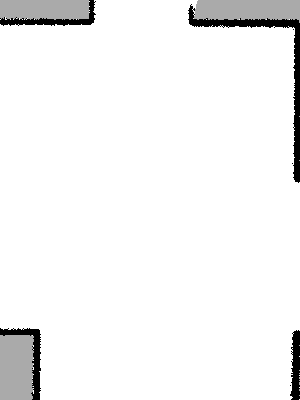
\includegraphics[scale=0.25]{cic_node_R}}
	\caption{Grade de ocupação do nó R}
	\label{fig:grade_no_R}
\end{figure}


\end{document}
